\section{Performance Evaluation}\label{sec:experiment}

\subsection{Experimental Result}

We have developed the client-side of Clockwork as a third-party framework (library) that can be readily used by mobile application developers, using Swift on the iOS platform as a proof-of-concept.  It is implemented using Java on the Amazon Web Service (AWS) platform. For the purpose of our real-world experiments, we have also developed a social messaging iOS application, using Facebook Parse (an MBaaS platform) as its backend, supported by our third-party framework. We identify $17$ different kinds of requests, such as \emph{send a message, send friend request, change username} and so on. We divide them into $K = 3$ types: type $3$ requests are the most urgent and type $1$ requests are the most delay-tolerant. 

To evaluate the performance of Clockwork, we carried out a pilot trial with $15$ iPhone users. We collected data for $20$ hours. Only the statistics regarding the request demand are logged, but not message contents, in order to protect user privacy.

\begin{figure}[t]
	\centering
	\hspace{-0.5cm}
	\begin{minipage}[t]{1.8in}
		\centering
		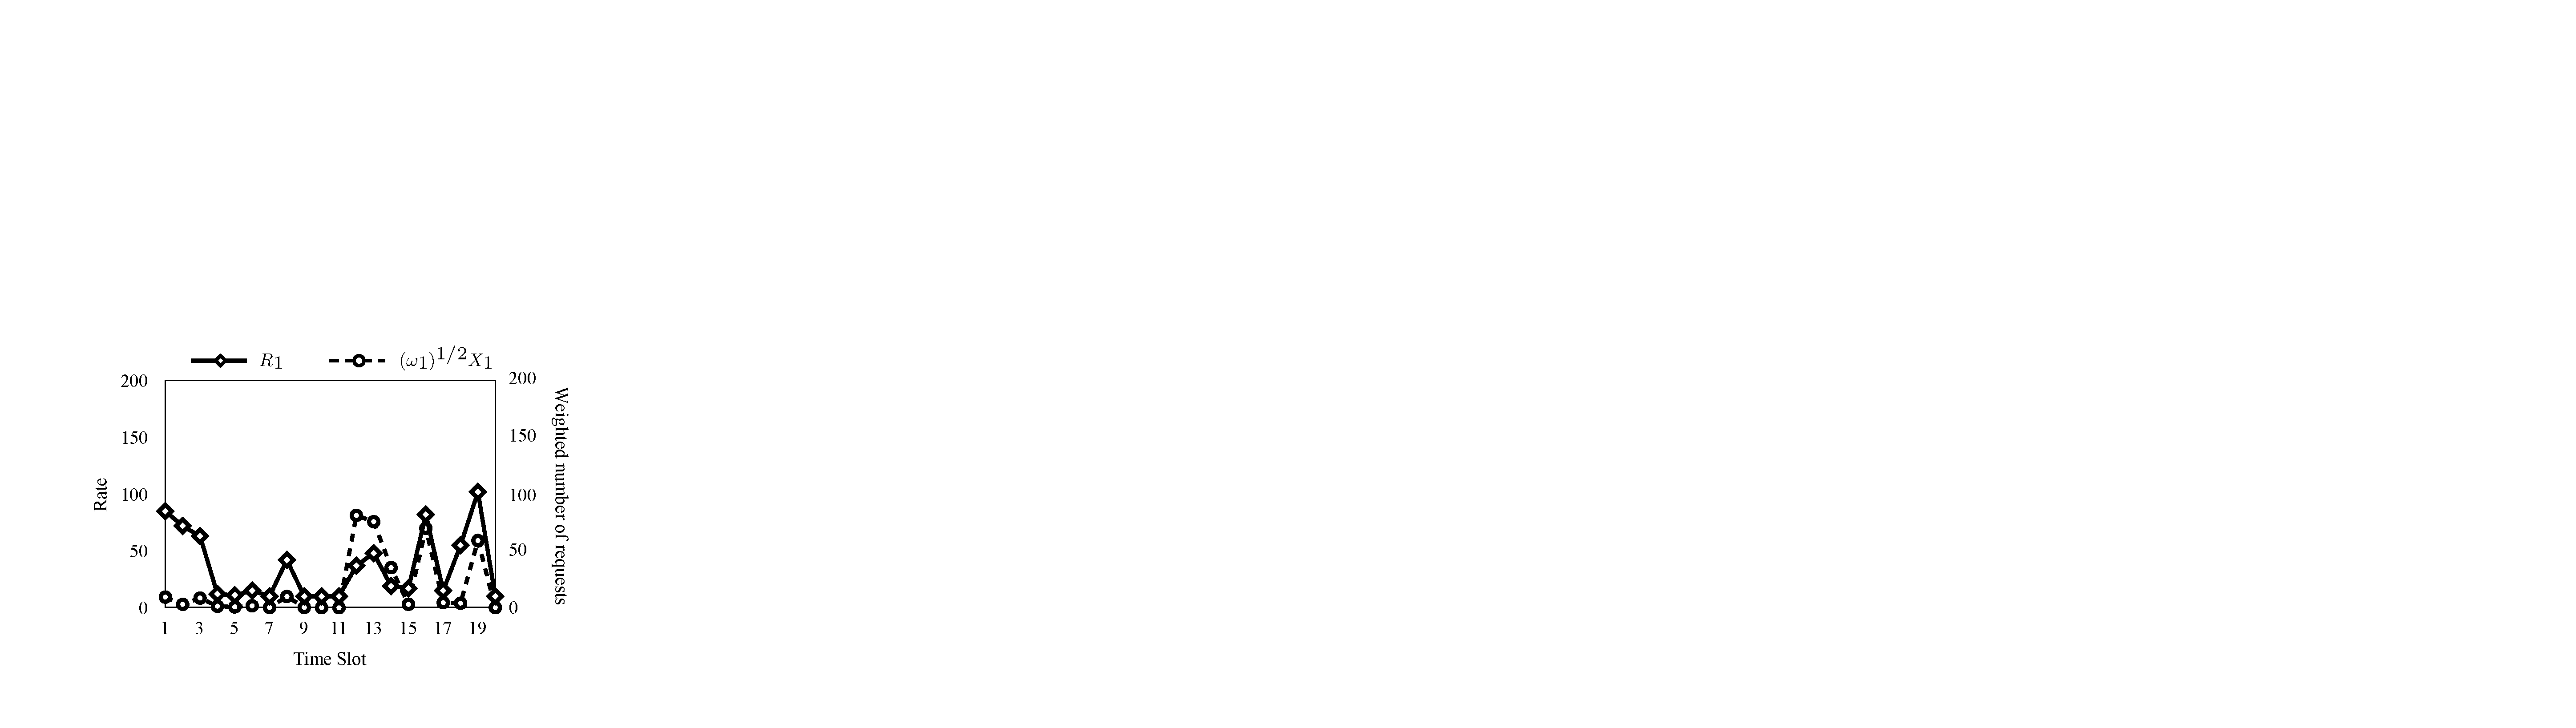
\includegraphics[trim=0mm 0mm 0mm 0mm, clip,width=1.8in]{figs/data1}\\
		\centerline{\small{(a) User 1}}
	\end{minipage}
	\hspace{-0.2cm}
	\begin{minipage}[t]{1.8in}
		\centering
		
\includegraphics[trim=0mm 0mm 0mm 0mm, clip,width=1.8in]{figs/data2}\\
		\centerline{\small{(b) User 2}}
	\end{minipage}
	\caption{Experimental result of rate allocation.} \label{fig:data}
\end{figure}

 \begin{figure}[t]
	\centering
	\hspace{-0.5cm}
	\begin{minipage}[t]{1.8in}
		\centering
		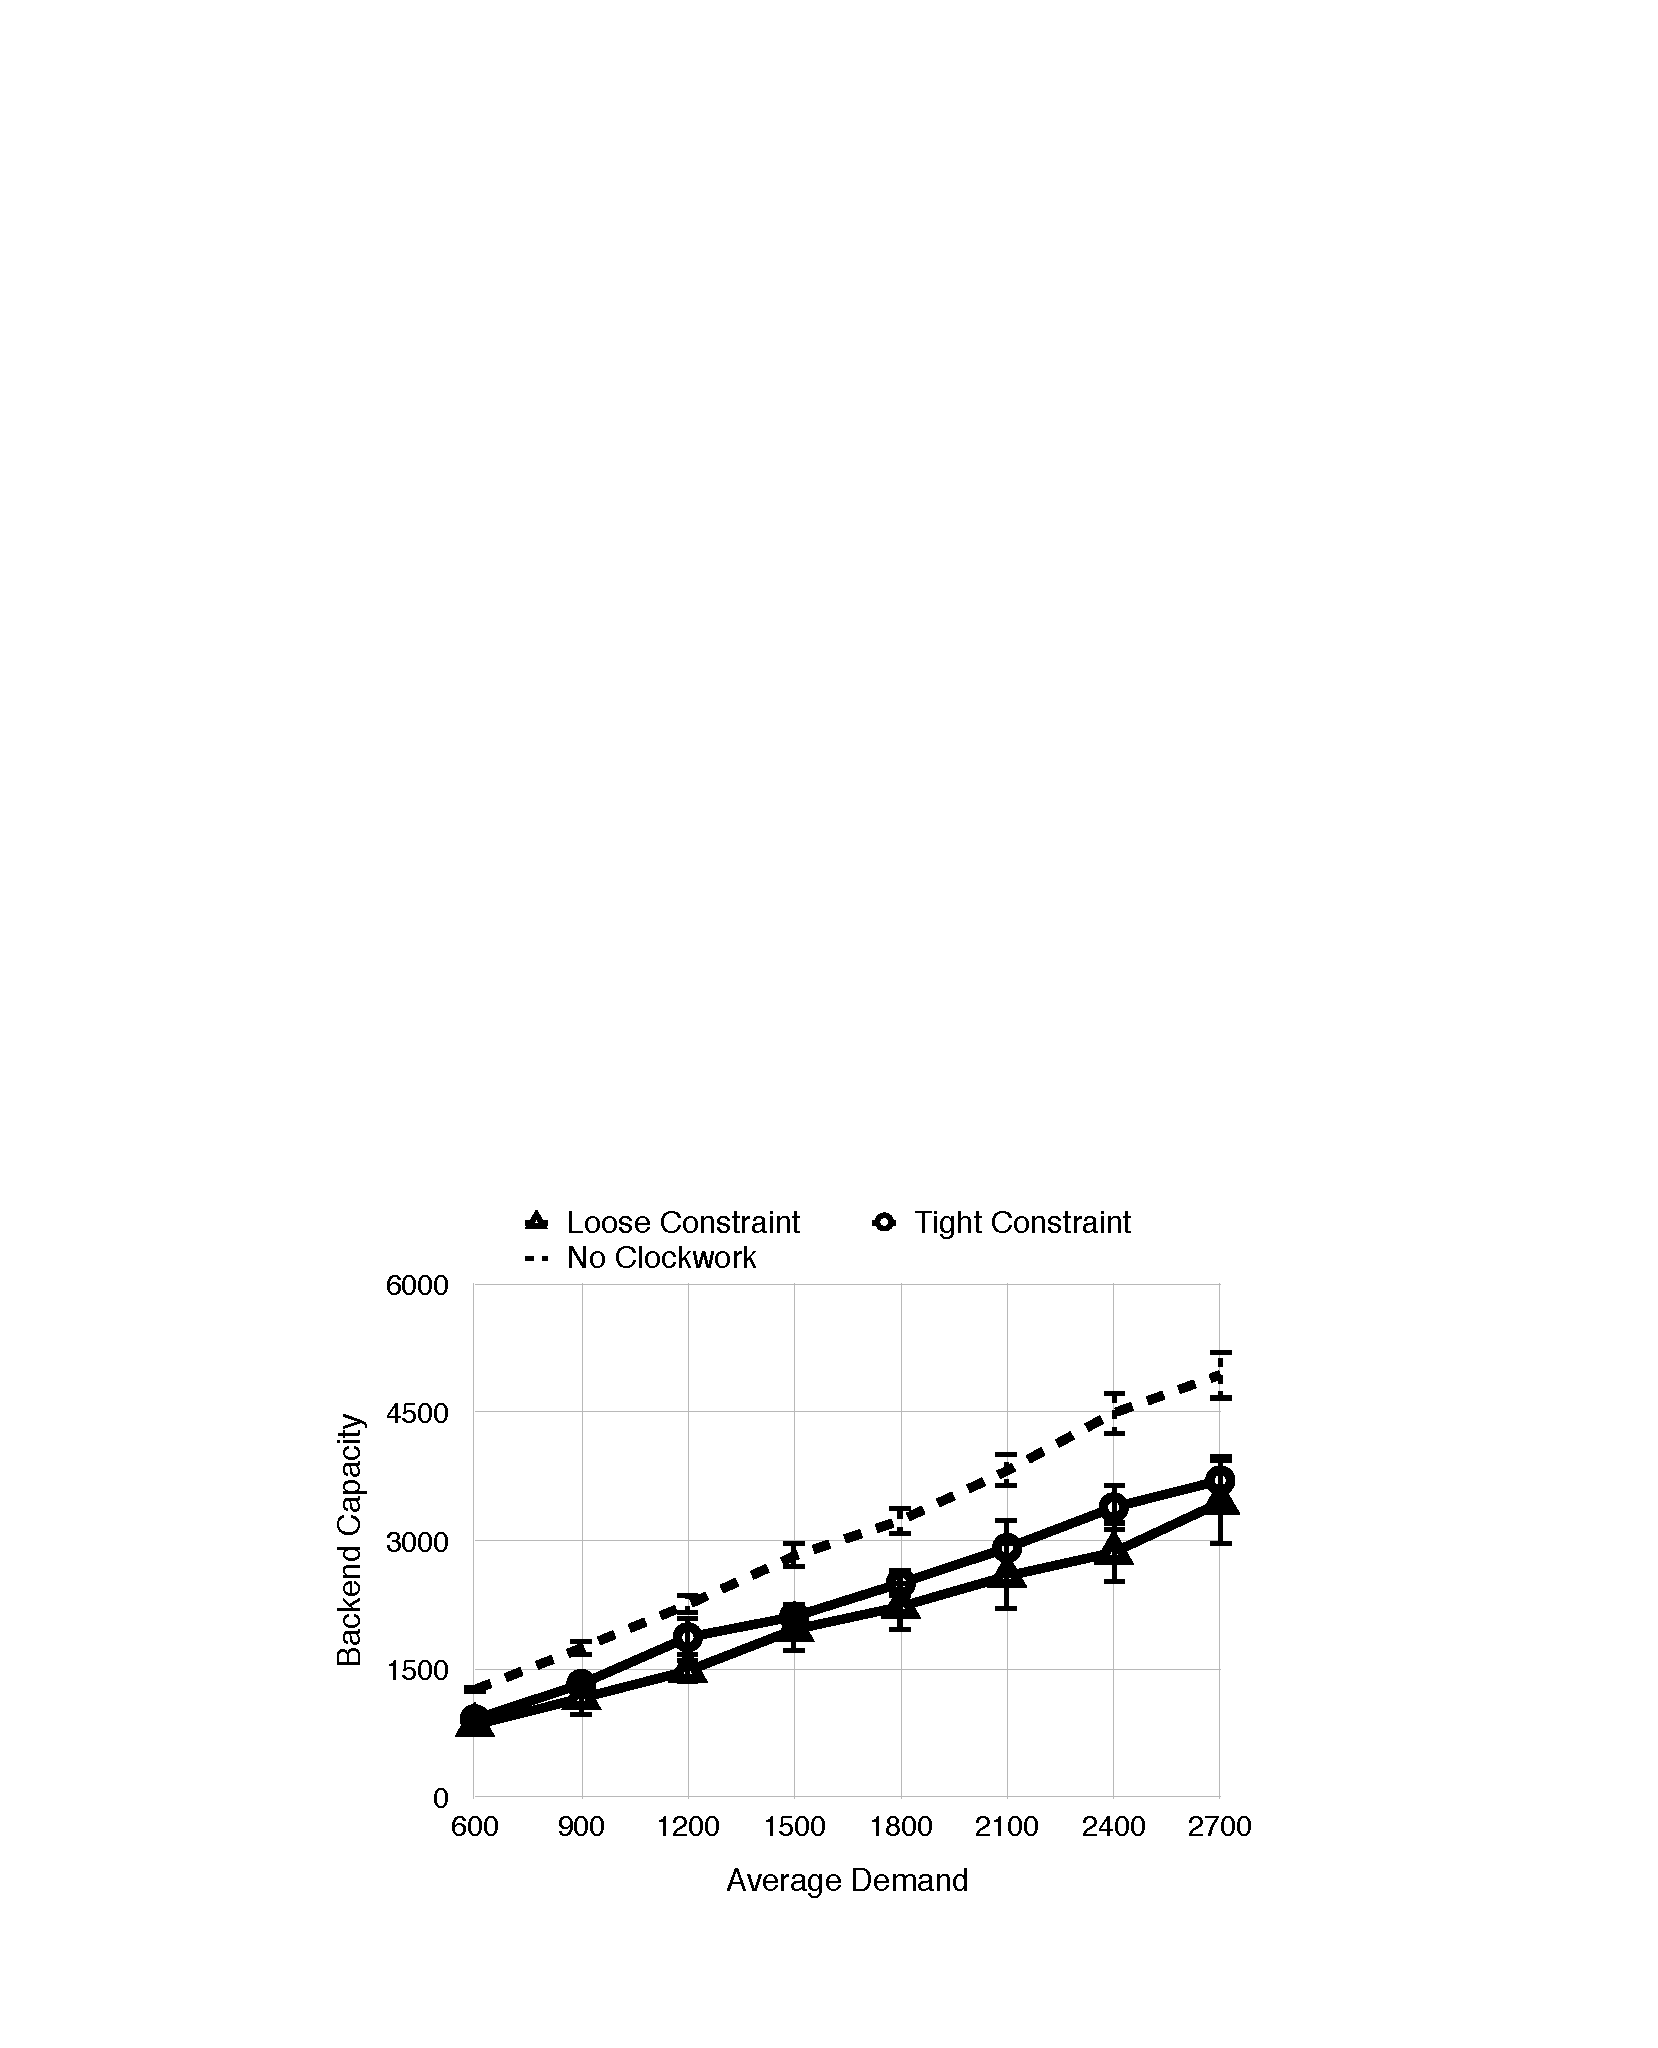
\includegraphics[trim=0mm 0mm 0mm 0mm, clip,width=1.8in]{figs/cp}\\
		\centerline{\small{(a) Required backend capacity}}
	\end{minipage}
	\hspace{-0.2cm}
	\begin{minipage}[t]{1.8in}
		\centering
		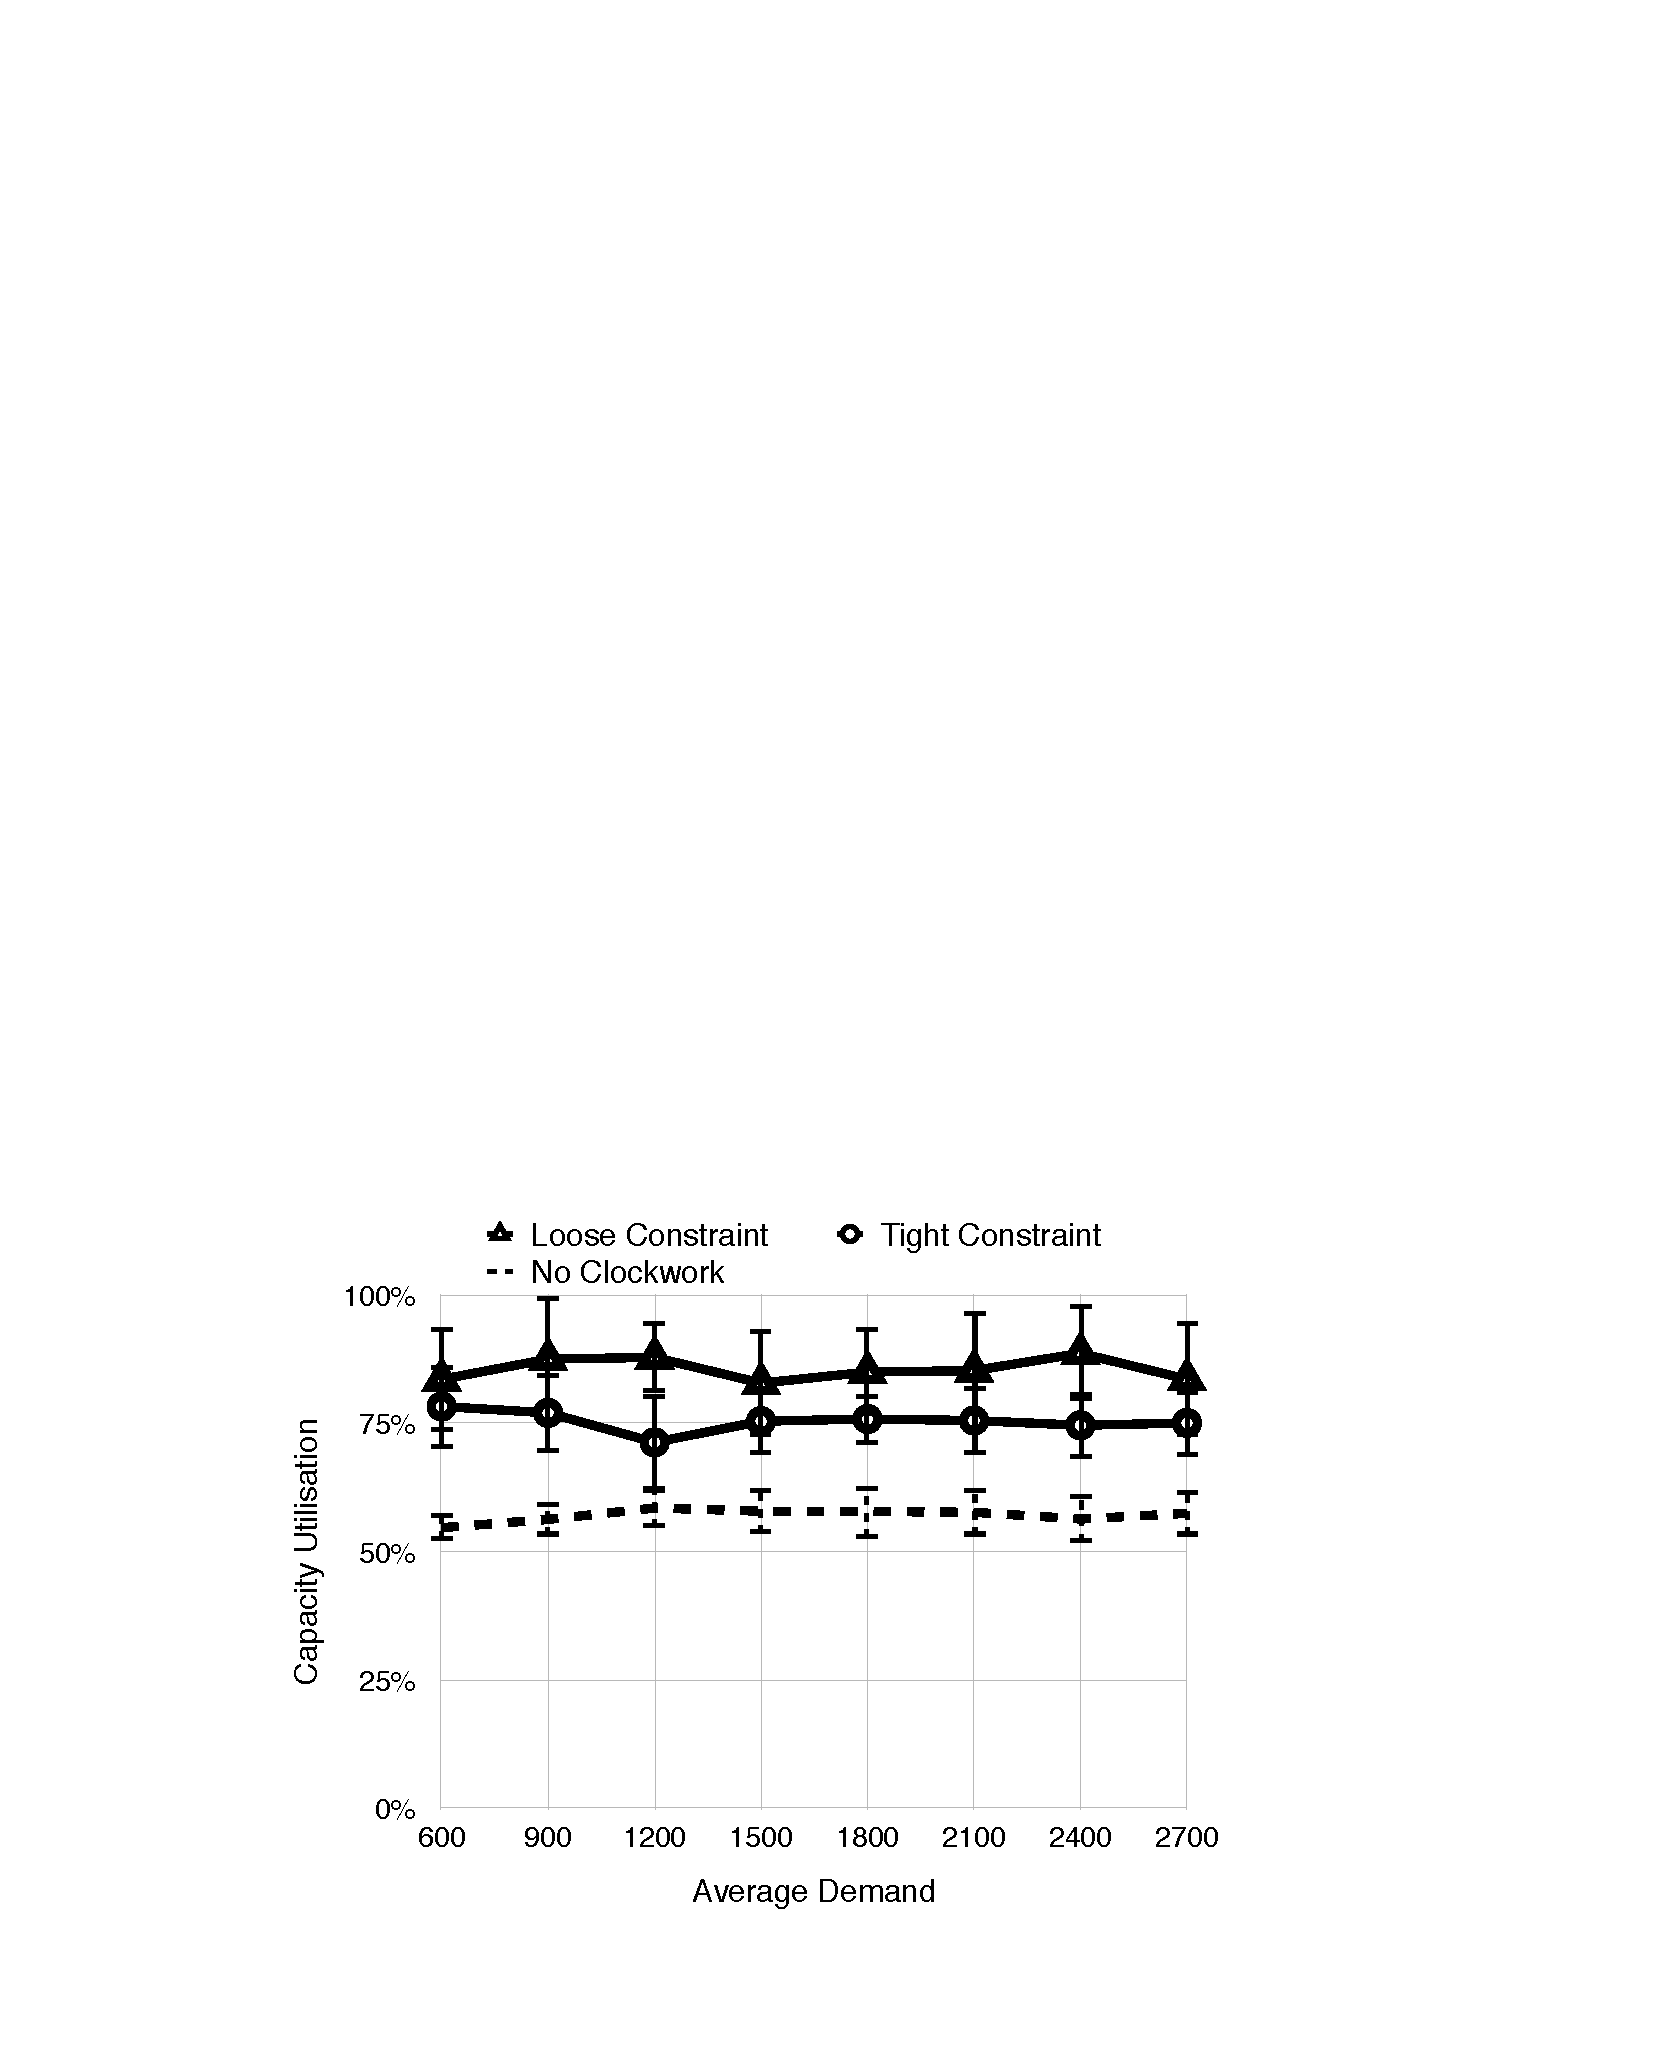
\includegraphics[trim=0mm 0mm 0mm 0mm, clip,width=1.8in]{figs/up}\\
		\centerline{\small{Backend capacity utilization}}
	\end{minipage}
	\caption{Simulation result of backend capacity planning.} \label{fig:serviceplan}
	\vspace{-1cm}
\end{figure}

\emph{Rate allocation}. We set $\alpha = 2$ in the $\alpha-$fair utility function, and show the rate allocation results of two users in Fig.~\ref{fig:data}. Generally speaking, a user will achieve a higher rate if her weighted number of requests is larger. Nevertheless, the allocated rate of a user also depends on the request demand of other users. For example, there is a plunge in user 1's request demand at time slot $15$, but the allocated rate is almost the same as that of the previous time slot. This is because the request demand of user 2 also falls dramatically at time slot $15$, making the ratio of the two users' request demand (i.e., $\frac{(\omega_1)^{1/2} X_1}{(\omega_2)^{1/2} X_2}$) in time slot $15$ approximately the same as that in time slot $14$. Thus, at time slot $15$, each user is assigned a rate similar to that in the previous time slot.

\emph{Capacity planning}. We use the collected data trace as inputs to the optimization problem (\ref{equ:opt}). We compare Clockwork and the baseline, where the backend capacity equals the peak demand. The backend utilization is calculated as the ratio of the average request demand to the backend capacity. The results are shown in Table~\ref{tab:exp}. With Clockwork, the backend cost for the developer can be reduced as much as $67.7\%$. Furthermore, Clockwork allows the developer to make a much better use of backend resources. Without Clockwork, the backend utilization is mostly below $50\%$, since the peak demand is much higher than the average demand. With Clockwork, the backend utilization can be increased  by as much as $76.8\%$. 

\begin{table}[t]
	\centering
	\caption{Experimental Result of Capacity Planning}
	\label{tab:exp}
	\begin{tabular}{|c|c|c|c|c|c|}
		\hline
		Hour & 1 &  2 & 3 & 4  &5\\
		\hline	
		Cost reduction &$67.7\%$ &$0.0\%$& $21.9\%$& $32.5\%$&$5.5\%$\\
		Utilization(baseline) &$20.3\%$ &$23.2\%$& $48.5\%$& $45.9\%$&$37.1\%$\\
		Utilization(Clockwork)&$63.0\%$ &$23.2\%$& $62.0\%$& $67.9\%$&$39.2\%$\\
		\hline
		Hour &6&7&8&9&10\\
		\hline
		Cost reduction&$31.3\%$ &$55.3\%$& $21.4\%$&$0.0\%$& $40.6\%$\\
		Utilization(baseline) & $39.2\%$ &$23.5\%$& $19.0\%$&$11.8\%$& $39.1\%$\\
		Utilization(Clockwork)&$57.0\%$ &$52.6\%$& $24.2\%$&$11.8\%$& $65.8\%$\\
		\hline
		Hour & 11 &  12  &13&14&15\\
		\hline
		Cost reduction &$63.0\%$ &$39.6\%$&$75.2\%$& $0.0\%$& $56.6\%$\\
		Utilization(baseline) & $18.6\%$ &$32.2\%$&$19.0\%$& $17.4\%$& $27.2\%$\\
		Utilization(Clockwork)&$50.3\%$ &$53.3\%$&$76.8\%$& $17.4\%$& $62.8\%$\\
		\hline
		Hour  & 16&17&18&19&20\\
		\hline
		Cost reduction &$23.4\%$ &$65.4\%$& $50.7\%$& $55.9\%$& $24.0\%$\\
		Utilization(baseline) & $44.4\%$ &$20.9\%$& $35.6\%$& $24.6\%$& $15.2\%$\\
		Utilization(Clockwork)&$57.9\%$ &$60.5\%$& $72.3\%$& $55.7\%$& $20.0\%$\\
		\hline
	\end{tabular}
	\vspace{-0.6cm}
\end{table}

\subsection{Simulation Result}
We evaluate the proposed backend capacity planning optimization model using a synthetic dataset generated as follows. There is a total of $100$ users, whose request generation processes follow independent and identical Poisson distributions.  We assume that there are $3$ types of requests. Type $3$ requests are most urgent, $\overline{\delta_{ij}^3}=0, \forall i,j$. No request is to be delayed for more than $5$ minutes, and the upper bounds for type $2$ and type $1$ requests are $\forall j-i\le 5, \overline{\delta_{ij}^2} =m-0.02*(j-i)$, and $\overline{\delta_{ij}^1} =m-0.01*(j-i)$, respectively. If $m$ is higher, more requests can be delayed, meaning that the constraint on request delay is looser, vice versa.

 It is shown in Fig.~\ref{fig:serviceplan}(a) that the backend capacity should augment with the average demand, but Clockwork can cut down the required backend capacity by as much as $36.3\%$. The capacity reduction is more significant under loose delay constraint ($m=0.4$) than under tight delay constraint ($m=0.1$). As shown in Fig.~\ref{fig:serviceplan}(b), provisioning for the peak demand will result in resource wastage as the backend capacity is underutilized for around $55\%$ at most of the time. With request scheduling of Clockwork, the demand profile becomes smoother, and the backend capacity can be utilized more efficiently. The improvement in the backend capacity utilization can be as high as $57.3\%$ under loose constraint, and $43.2\%$ under tight constraint.
 



